\documentclass[a4paper,11pt]{book}

\usepackage[T1]{fontenc}
\usepackage[utf8]{inputenc}
\usepackage[LGR,T1]{fontenc} % notice LGRx instead of LGR
\usepackage{lmodern}
\usepackage[final]{pdfpages} 
\usepackage[top=2cm, bottom=3cm, outer=3cm, inner=4cm, headsep=14pt]{geometry}
\usepackage{textgreek}
\usepackage{csquotes}
\usepackage[french]{babel}
\usepackage{fancyhdr}
\usepackage{xsim}
\usepackage{tasks}
\usepackage[absolute]{textpos}
\usepackage{ascii}
\usepackage{eurosym}
\usepackage{amsthm}
\usepackage{url}

\theoremstyle{definition}
\newtheorem{exmp}{Example}[section]

\bibliographystyle{abbrv}
\pagestyle{fancy}
\fancyhf{}
\renewcommand{\footrulewidth}{1pt}
\renewcommand{\thesection}{\arabic{section}}

\lhead{Architecture des ordinateurs}
\rhead{Semi-Conducteurs}
\rfoot{Page \thepage}

\begin{document}

\chapter{Semi-Conducteurs}
\section{Généralités}
Dans un atome, les électrons sont organisés en bandes d'énergie autour du noyau. Un matériau conducteur possède pour les couches externes :
\begin{itemize}
    \item Une bande de valence qui est complète.
    \item Une bande de conduction qui est partiellement remplie. Cette couche contient donc quelques électrons qui participent au courant électrique.
\end{itemize}
De plus, pour être conducteur, il faut que ces deux bandes se superposent, ce qui permet la circulation des électrons dans le solide.
Dans le cas des semi-conducteurs, l'espace "interdit" qui sépare ces deux bandes est relativement faible et permet donc aux électrons de circuler à certaines conditions de température et d'énergie transmise aux électrons sous forme de champs électrique.

\section{Le silicium mono-cristallin}
Le silicium mono-cristallin est un semi-conducteur obtenu à des températures d'environ $1'700^o$. Un atome de silicium possède quatre électrons sur huit dans la dernière bande. Dans le réseau mono-cristallin  obtenu, les atomes de silicium ont chacun quatre voisins liés par des liaisons covalantes. Dans cette configuration, tous les électrons sont utilisés dans les liaisons, et le courant ne peut plus passer. On retrouve une situation similaire dans la bande suivante avec le germanium (voir figure \ref{fig:period}). 

\begin{figure}[h]
\centering
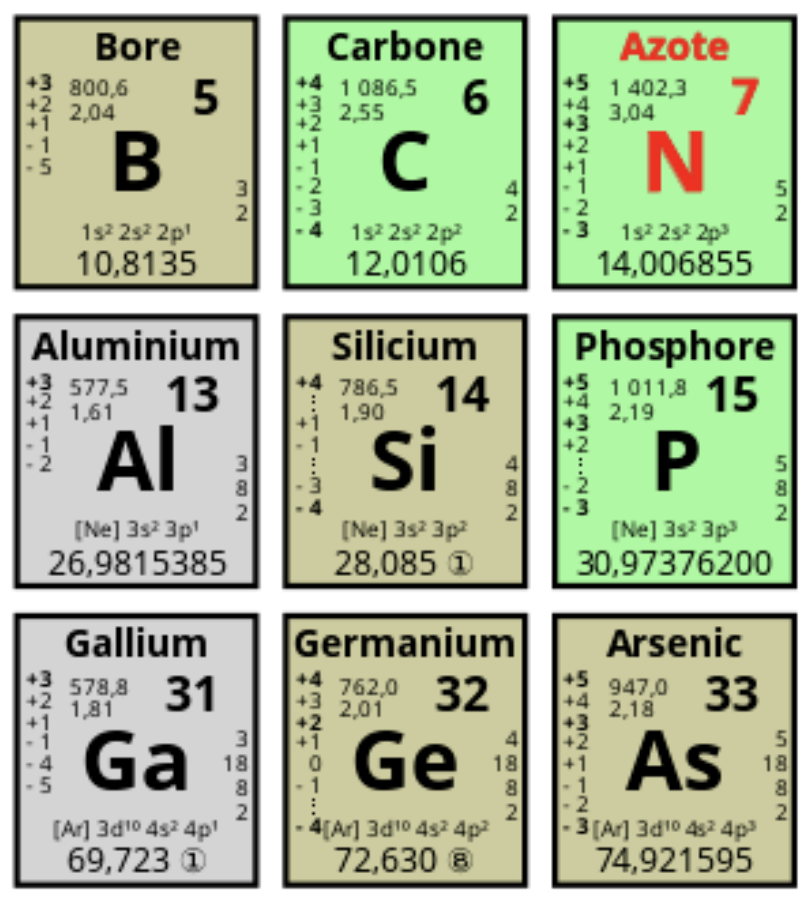
\includegraphics[width=0.5\textwidth]{media/Semicon/TabPerioSI.png}
\caption{Le Silicium et le Germanium dans le tableau périodique}
\label{fig:period}
\end{figure}

\section{Silicium dopé}
On peut introduire des atomes d'un autre élément dans le silicium mono-cristallin (sans détailler ici le processus). On peut ajouter des atomes de phosphore dans le cristal de silicium. Cela ajoute un des électrons libres en excédents qui peuvent voyager, et l'on obtient un courant. Le silicium ainsi dopé devient conducteur (figure \ref{fig:dopageN}).

\begin{figure}[h]
\centering
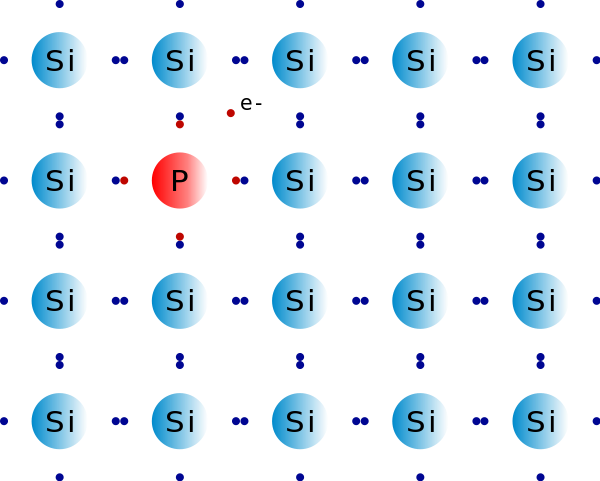
\includegraphics[width=0.5\textwidth]{media/Semicon/600px-N-doped_Si.svg.png}
\caption{Dopage N}
\label{fig:dopageN}
\end{figure}
On parle de dopage N. On peut aussi utiliser de l'arsenic pour le dopage.

De manière symétrique, on peut doper le silicium avec de l'aluminium (ou du Bore) pour obtenir un dopage P, avec un déficit d'électrons (figure \ref{fig:dopageP}).

\begin{figure}[h]
\centering
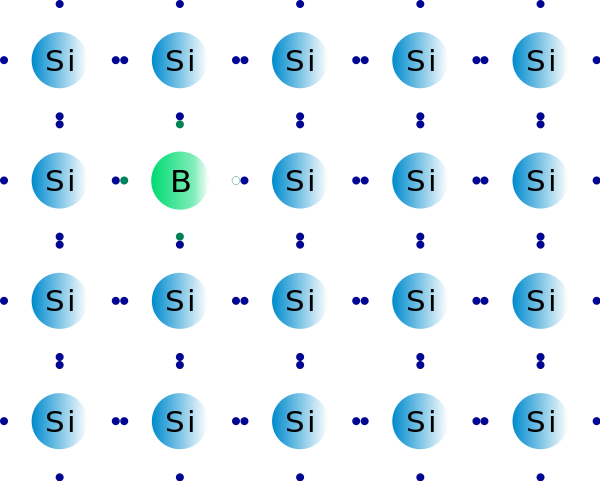
\includegraphics[width=0.5\textwidth]{media/Semicon/600px-P-doped_Si.svg.png}
\caption{Dopage P}
\label{fig:dopageP}
\end{figure}

Là aussi, le silicium devient conducteur.

\section{Jonction P-N et diode}
On obtient une jonction P-N lorsque l'on met en contact une zone P avec une zone N. En principe, il s'agit du même substrat de silicium mono-cristallin dopé d'une part en mode P, d'autre part en mode N. Il se forme à la jonction une zone de \emph{déplétion}. Cela se traduit par une migration des électrons de la zone où ils sont en excès vers la zone où ils sont en déficit. Cela crée une zone ou il n'y a plus de porteurs libres, c'est-à-dire plus d'électrons disponibles pour établir un courant. Cette zone a les mêmes propriétés que le silicium pur (non-conducteur).

Si on applique une tension en polarisation directe, comme sur la figure \ref{fig:forward}, les charges libres regagnent la partie N de la zone de déplétion et inversement, le déficit est repoussé du côté P. À partir d'une certaine tension, la zone de déplétion disparaît et le courant peut à nouveau circuler.

\begin{figure}[h]
\centering
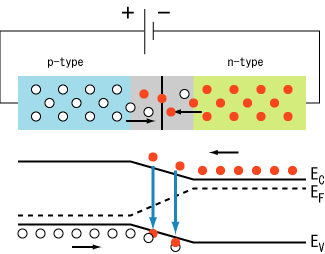
\includegraphics[width=0.5\textwidth]{media/Semicon/PnJunction-Diode-ForwardBias.png}
\caption{Polarisation directe (source: Wikipedia)}
\label{fig:forward}
\end{figure}

À l'inverse, si on applique une tension en polarisation inverse, la zone de déplétion s'agrandit et le milieu devient fortement isolant jusqu'à une tension dite d'effondrement. Ceci est illustré sur la figure \ref{fig:reverse}.

\begin{figure}[h]
\centering
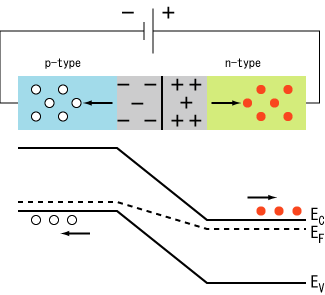
\includegraphics[width=0.5\textwidth]{media/Semicon/PnJunction-Diode-ReverseBias.png}
\caption{Polarisation inverse (source: Wikipedia)}
\label{fig:reverse}
\end{figure}

Ce dispositif est à la base la diode, un composant électronique qui laisse passer le courant dans un sens mais pas dans l'autre. Lorsque la tension est suffisante en polarisation directe, le courant passe avec, éventuellement, émission de photons dans le cas des DEL. Cette tension en polarisation directe dépend des matériaux utilisés et de différentes caractéristiques de la diode, mais elle est très fréquemment de 0.7V.

\section{Les transistors bipolaires}
On obtient un transistor bipolaire en assemblant trois couches selon le schéma N-P-N ou P-N-P, c'est-à-dire en composant  deux jonctions inverses, comme illustré sur la figure \ref{fig:NPN_PNP}. 

Dans cette configuration, la jonction base - émetteur est appelée jonction de commande. Un faible courant base - émetteur, ou simplement courant de base, appelé aussi courant de commande, permet le passage d'un courant plus important entre le collecteur et l'émetteur avec la relation :
\[ I_C = \beta I_B   \]

Où l'on a $\beta$ le gain en courant du transistor.

Le composant fonctionne comme si la résistance entre l'émetteur et le collecteur variait en fonction du courant de commande $I_B$, d'où le nom \textbf{Transistor} contraction de \emph{Transfert resistor}.

\begin{figure}
\centering
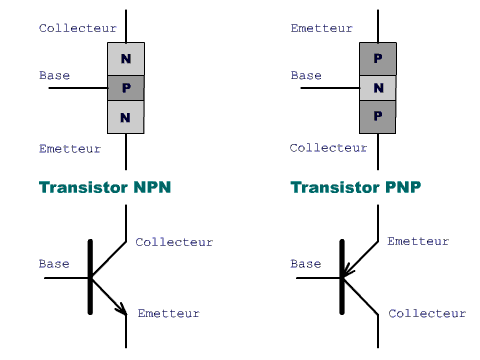
\includegraphics[width=0.5\textwidth]{media/Semicon/NPN_PNP.png}
\caption{Transistors NPN et PNP (Source : courstechinfo.be)}
\label{fig:NPN_PNP}
\end{figure}

On trouvera une introduction à l'électronique du transistor bipolaire dans la vidéo \cite{transistor}.

\section{Les transistors à effet de champ}
Les transistors FET\footnote{FET : Field Effect Transistor} sont constitués d'un canal Source-Drain relativement étroit qui est conducteur de base. Une Grille est posée sur le canal comme on peut le voir sur la figure \ref{fig:FET}. On parle aussi de transistor unipolaire puisque le canal source - drain est composé d'un seul type de porteurs de charges mobiles.
Nous n'allons pas détailler dans cette rapide introduction le fonctionnement des transistors FET. Le principe de base consiste dans le fait que l'application d'une tension inverse entre la Grille (Gate en anglais) et la source va créer une zone isolante (agrandissement de la zone de déplétion) dans le canal Source-Drain, comme on peut le voir sur la figure \ref{fig:FET_N}

\begin{figure}
\centering
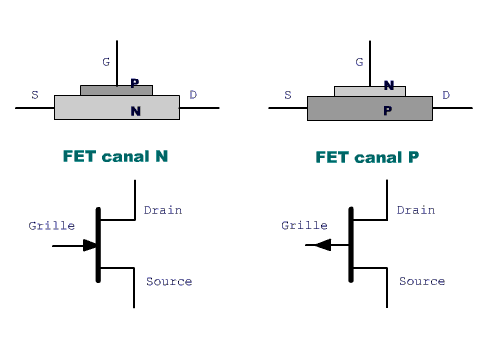
\includegraphics[width=0.5\textwidth]{media/Semicon/FET_N_et_P.png}
\caption{Transistors FET (Source : courstechinfo.be)}
\label{fig:FET}
\end{figure}

\begin{figure}
\centering
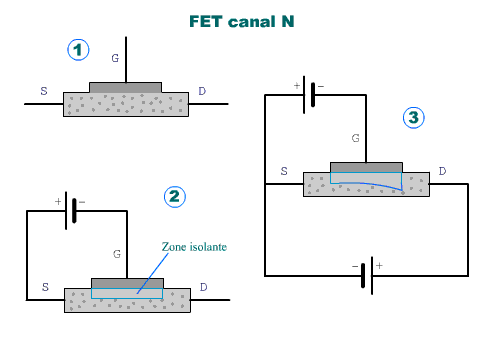
\includegraphics[width=0.5\textwidth]{media/Semicon/FET_N.png}
\caption{Transistors FET N avec une tension de commande inverse (Source : courstechinfo.be)}
\label{fig:FET_N}
\end{figure}

Les transistors à effet de champ, comme décrits ici, sont surtout utilisés pour des applications analogiques. Notons pour l'anecdote que le premier brevet décrivant le transistor à effet de champ date de 1925 (Julius E. Lilienfeld), mais c'est en 1952 qu'il sera finalement redécouvert par Kahng et Atalla.

\section{Transistors MOSFET}
Les transistors MOSFET concurrencent éfficacement les transistors bipolaires, en particulier dans le cas des circuits intégrés numériques.

Dans un MOSFET, la Grille (Gate), en aluminium, est séparée du substrat par un isolant, du SiO2, comme on peut le voir sur la figure \ref{fig:MOSFET}.

\begin{figure}
\centering
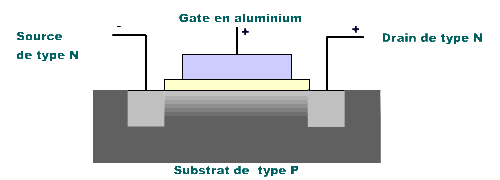
\includegraphics[width=0.5\textwidth]{media/Semicon/MOSFET.png}
\caption{Transistor MOSFET(Source : courstechinfo.be)}
\label{fig:MOSFET}
\end{figure}

Le fonctionnement est relativement similaire à celui décrit plus haut pour le FET. Il ne nécessite aucun courant pour le commander, uniquement une tension sur la Grille. Il est particulièrement adapté pour les circuits intégrés comme les microprocesseurs et la mémoire.

Il existe différents types de MOSFET, sans entrer dans les détails dans cette introduction rapide aux transistors, nous donnons juste les différents schémas possibles dans les figures \ref{fig:EMOS} et \ref{fig:DMOS}. 

\begin{figure}
\centering
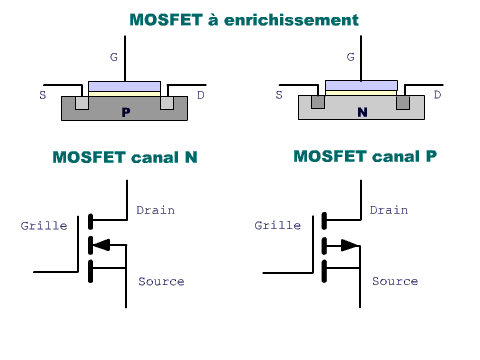
\includegraphics[width=0.5\textwidth]{media/Semicon/EMOS.png}
\caption{Transistor MOSFET à enrichissement (Source : courstechinfo.be)}
\label{fig:EMOS}
\end{figure}

\begin{figure}
\centering
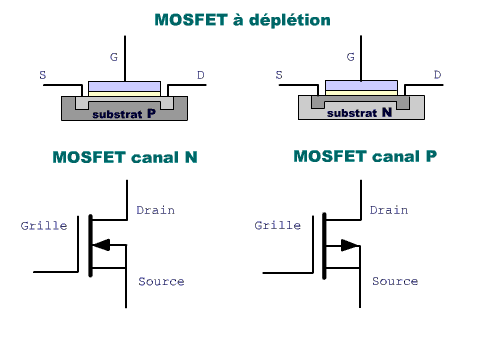
\includegraphics[width=0.5\textwidth]{media/Semicon/DMOS.png}
\caption{Transistor MOSFET à déplétion (Source : courstechinfo.be)}
\label{fig:DMOS}
\end{figure}

Pour trouver plus d'explications, on se rendra sur \cite{semiconducteurs} et pour d'autres types de transistors sur \cite{effetdechamp}.


%\bibliography{biblio.bib}


\end{document}

